\chapter{蛋白质结构生物学}\label{ch:b3:structural-biology}

马克斯·佩鲁茨于 1937 年开始研究血红蛋白的结构，
并于 1960 年发表成果：前后历时二十二年，以半
纳米的\omterm{def:b3:structural-biology:methods}{分辨率}看清四条各含 150 个氨基酸的肽链如何
环绕四个血红素折叠。一个血红蛋白分子只需
几毫秒便能自行折叠。这两个事实之间，即本章的主题：
蛋白质的结构是什么，为何氨基酸链会呈现这一形状而非
另一种形状，它又如何在天文数字般的备选构象中如此迅速地找到
这一形状，出错时又会怎样，
这些形状如何被观测——借助 X 射线、磁共振、电子，
乃至如今的计算——以及蛋白质如何在不同形状之间
移动以完成其功能，血红蛋白在紧张态与松弛态之间的转换，
此后便成为所有别构蛋白的模型。

\section{蛋白质的结构是什么}

\begin{definition}[结构的层次]\label{def:b3:structural-biology:levels}
\index{二级结构}\index{α 螺旋}\index{β 折叠}\index{三级结构}\index{结构域}\index{折叠类型}
\emph{一级结构}是残基的序列。
\emph{二级结构}是主链局部的规则构象，
由主链羰基与酰胺基之间的氢键稳定，
其中\emph{$\alpha$ 螺旋}为右手螺旋，每圈含 $3.6$
个残基，每残基上升 \qty{0.15}{nm}（\qty{0.54}{nm}
每圈），每个羰基与其后第四个残基的酰胺基成键；以及
\emph{$\beta$ 折叠}由伸展的链段并排排列而成，
可平行或反平行，并与相邻链成键，侧链
交替位于折叠片层的上下两侧。\emph{三级结构}是
整条链在三维空间中的折叠方式；蛋白质链中一个紧凑、可独立折叠的
单元，含 \numrange{50}{250} 个残基，称为\emph{结构域}，
结构域中二级结构元件的排列即其\emph{折叠类型}。
\emph{四级结构}是由若干条链\omterm{def:b3:genomics:assembly}{组装}而成的结构：
血红蛋白的 $\alpha_{2}\beta_{2}$。约 \num{1300} 种折叠类型可涵盖全部已知结构域，
而其中数十种——罗斯曼折叠、
TIM 桶、免疫球蛋白折叠等——它们便涵盖了
大部分蛋白质：自然界反复利用折叠类型，并使其序列各异。
\end{definition}

\begin{omfigure}
\begin{tikzpicture}
\begin{axis}[
  width=6.4cm, height=6.4cm,
  xmin=-180, xmax=180, ymin=-180, ymax=180,
  xlabel={$\phi$（度）}, ylabel={$\psi$（度）},
  xlabel style={font=\small}, ylabel style={font=\small},
  tick label style={font=\scriptsize}, xtick={-180,-90,0,90,180}, ytick={-180,-90,0,90,180},
  axis lines=box, grid=major, grid style={gray!25},
  clip=false,
]
% beta region
\fill[omDef!30] (axis cs:-180,90) rectangle (axis cs:-45,180);
\fill[omDef!30] (axis cs:-180,-180) rectangle (axis cs:-45,-150);
\node[font=\scriptsize, omDef!60!black] at (axis cs:-112,165) {$\beta$ 链};
% alpha R region
\fill[omThm!30] (axis cs:-160,-70) rectangle (axis cs:-45,0);
\node[font=\scriptsize, omThm!70!black] at (axis cs:-105,-58) {右手 $\alpha$};
% alpha L region
\fill[omMeth!30] (axis cs:45,0) rectangle (axis cs:100,80);
\node[font=\scriptsize, omMeth!60!black, align=center] at (axis cs:72,40) {左 \\手性};
\addplot[only marks, mark=*, mark size=1pt, black] coordinates {(-57,-47)};
\node[font=\scriptsize, anchor=south west] at (axis cs:-52,-44) {$\alpha$：$(-57,-47)$};
\addplot[only marks, mark=*, mark size=1pt, black] coordinates {(-139,135)};
\node[font=\scriptsize, anchor=west] at (axis cs:-134,135) {反平行 $\beta$};
\end{axis}
\node[align=left, font=\scriptsize, anchor=west] at (7.0,3.0) {每个残基的两个主链扭转角 \\$\phi$（绕 N--C$_\alpha$）与 $\psi$（绕 C$_\alpha$--C）\\受空间位阻限制，只能落在着色区域内。\\螺旋中每个残基都落在同一点附近；\\链段则靠近另一区域。\\甘氨酸无侧链，可伸展得更远；\\脯氨酸因带有环状结构，\\固定在 $\phi = -60$ 附近。};
\end{tikzpicture}

{\small 拉马钱德兰图。阴影区域为空间位阻所允许的
主链角 $\phi$ 与 $\psi$ 的组合；
右手 $\alpha$ 螺旋与 $\beta$ 链各对应一个
小区域，折叠蛋白质的大多数残基落入其中
之一。}
\end{omfigure}

\begin{proposition}[维持折叠的作用力]\label{prop:b3:structural-biology:forces}
\index{疏水效应}\index{边际稳定性}
折叠后的蛋白质由\emph{\omterm{prop:b3:structural-biology:forces}{疏水效应}}稳定——
即将非极性侧链埋入远离水的核心，使
原本会在其周围有序排列的水分子得以释放；
此外还有\omterm{def:b3:structural-biology:levels}{二级结构}及埋藏极性基团所形成的氢键，
核心中如晶体般致密的范德华堆积，
偶尔的盐桥，以及分泌蛋白中的二硫
键。\omterm{prop:b3:structural-biology:forces}{疏水效应}提供了折叠的大部分驱动力；氢键
大多能自我补偿（未折叠时与水成键的主链，
在折叠态中则与自身成键），而是
决定\emph{哪种}折叠方式。折叠的净自由能很小，
$\Delta G \approx -20$ 至 \qty{-60}{kJ/mol}——仅相当于
几个氢键的强度（对拥有数百个氢键的分子而言），原因在于
折叠时构象熵的损失几乎抵消了
焓的增益。蛋白质是\emph{边际稳定}的：几度的温度变化、
pH 的改变或核心中的一个突变都可使其展开，这种
边际性正是它们得以运动的原因。
\end{proposition}

\begin{proof}[实验证据]
安芬森（1961）用尿素和还原剂使核糖核酸酶~A 展开，
打断其四个二硫键，活性随之丧失；去除
二者后，酶重新折叠，于 $105$ 种可能的
二硫键配对中重新形成正确的四个，并恢复全部活性。无模板、
无酶，亦无序列之外的信息存在：天然结构
是肽链可达到的热力学最稳定状态，
而序列编码了它。于肽链仍处于尿素中时，将二硫键
重新氧化，得到杂乱的混合物，其活性
仅为 \qty{1}{\%}，此后在允许折叠时重排为天然形式：
即肽链自行找到了能量最低点。
\end{proof}

\section{肽链如何找到其折叠类型}

\begin{theorem}[莱文索尔悖论]\label{thm:b3:structural-biology:levinthal}
\index{莱文索尔悖论}\index{折叠漏斗}
若蛋白质的 $n$ 个残基各自可独立采取 $k$ 种主链
构象，则该链共有 $k^{n}$ 种构象。
当 $k = 3$、$n = 100$ 时，即 $3^{100} \approx
5\times 10^{47}$；若每皮秒取样一种（每秒 $10^{12}$
种），则需 $5\times 10^{35}$ 秒，约 $10^{28}$ 年。
此大小的蛋白质在毫秒至秒之间即可折叠。因此
折叠并非随机搜索构象：能量
面是一个\emph{漏斗}，其中几乎每一个局部构象
都偏向天然状态，肽链通过局部
移动而下降，每一步平均而言都是下坡的。
\end{theorem}
\begin{proof}
计数即乘法原理；所需时间即计数
除以取样速率，即 $5\times 10^{47}/10^{12} = 5\times
10^{35}$ 秒，一年约为 $3\times 10^{7}$ 秒。结论即
逆否命题：此规模的随机搜索在
观测时间内是不可能的，故搜索并非随机。使其非随机的
原因在于：链某一部分形成的相互作用持续存在，
而其他部分仍在形成（疏水塌缩与螺旋形成
在微秒内发生，并缩小了待搜索的空间），以及部分
正确的结构平均能量低于错误结构，因此
下降过程受到引导——是一个漏斗，而不是
只有一个洞的高尔夫球场。
\end{proof}

\begin{omfigure}
\begin{tikzpicture}[every node/.style={font=\scriptsize}, >=stealth]
  % funnel outline
  \draw[very thick, omDef] (-4,3) .. controls (-3.2,1.5) and (-1.2,0.2) .. (-0.35,-1.2) -- (-0.35,-1.6);
  \draw[very thick, omDef] (4,3) .. controls (3.2,1.5) and (1.2,0.2) .. (0.35,-1.2) -- (0.35,-1.6);
  \draw[very thick, omDef] (-0.35,-1.6) -- (0.35,-1.6);
  % rugged inner lines
  \draw[omDef!60, thick] (-3.3,2.6) .. controls (-2.9,2.2) and (-2.6,2.6) .. (-2.2,2.0) .. controls (-1.9,1.5) and (-1.7,1.9) .. (-1.4,1.2) .. controls (-1.1,0.7) and (-0.9,0.9) .. (-0.6,0.2);
  \draw[omDef!60, thick] (3.3,2.6) .. controls (2.9,2.1) and (2.5,2.5) .. (2.1,1.8) .. controls (1.8,1.3) and (1.5,1.6) .. (1.2,1.0) .. controls (1.0,0.6) and (0.8,0.8) .. (0.6,0.2);
  % axes
  \draw[->] (-5.9,-1.8) -- (-5.9,3.2) node[above, align=center] {自由 \\能};
  \draw[<->] (-3.9,3.85) -- (3.9,3.85) node[midway, above] {构象熵（构象系综的宽度）};
  % labels
  \node[above] at (0,3.05) {未折叠链：构象多，能量高};
  \node[right, align=left] at (3.3,1.4) {局部陷阱：部分 \\错误折叠的中间产物};
  \node[left, align=right] at (-3.3,1.4) {快速塌缩与 \\二级结构};
  \node[below] at (0,-1.7) {天然态：构象唯一，能量最低};
  \draw[->, thick, omThm] (-2.8,2.4) .. controls (-2.0,1.2) and (-0.8,0.5) .. (-0.15,-1.3);
  \node[omThm, left] at (-1.5,-0.5) {一条折叠轨迹};
\end{tikzpicture}

{\small \omterm{thm:b3:structural-biology:levinthal}{折叠漏斗}。链趋近天然态时，自由能下降，
可用构象的数目减少；漏斗壁崎岖，
链可能被困在部分错误折叠的
中间产物中，但总体斜坡仍会在
毫秒内将其带下去。}
\end{omfigure}

\begin{definition}[分子伴侣]\label{def:b3:structural-biology:chaperones}
\index{分子伴侣}\index{Hsp70}\index{伴侣蛋白}\index{GroEL}
\emph{分子伴侣}是一类协助其他蛋白质折叠的蛋白质，
它本身并不构成这些蛋白质的一部分，也不提供关于折叠方式的信息：
它阻止聚集，而聚集会在拥挤的细胞质中与折叠相竞争。
\emph{Hsp70}结合暴露在外的疏水片段，
这些片段来自新生链或未折叠链，通过 ATP 水解将其释放，
以便再次尝试。\emph{伴侣蛋白} GroEL（线粒体中为 Hsp60，
真核细胞的细胞溶胶中为 TRiC）是由十四个亚基组成的双桶状结构，
其中央空腔由 GroES 封盖，可容纳分子量至多
\qty{60}{kDa} 的单链，单独包裹约十秒钟——一个安芬森笼
——随后不论是否折叠都将其释放，使其再试。约十分之一
新合成的细菌蛋白质会经过 GroEL。若细胞的
分子伴侣不堪重负——例如受热（这正是大多数分子伴侣
成为\emph{热激蛋白}的原因，由温度升高所诱导）——细胞
充满聚集体。
\end{definition}

\begin{definition}[淀粉样蛋白]\label{def:b3:structural-biology:amyloid}
\index{淀粉样蛋白}\index{交叉 β}\index{朊病毒}\index{错误折叠疾病}
\emph{淀粉样蛋白}是一种有序的蛋白质聚集体，其中的链
堆叠成不分支的纤维，纤维宽 \qtyrange{5}{10}{nm}，
每条链的链段垂直于纤维轴排列，并与
下一条链的链段形成氢键——这就是\emph{交叉$\beta$}结构，
无论是哪种蛋白质，其结构都相同。几乎任何蛋白质在失稳条件下都能形成它；
在\emph{错误折叠疾病}中，特定蛋白质会在体内这样做：
淀粉样 $\beta$ 蛋白和 tau 蛋白与阿尔茨海默
病有关，$\alpha$-突触核蛋白与帕金森病有关，亨廷顿蛋白、转甲状腺素蛋白，
以及 2 型糖尿病中的胰岛淀粉样多肽。\emph{朊病毒}是一种能够自我传播的淀粉样蛋白：
朊病毒蛋白 PrP 的错误折叠形式
接触时将正常形式转化为更多自身，因此这种“感染”
不携带核酸，只携带一种构象——这一机制见于羊瘙痒病、
牛海绵状脑病与克雅氏病，
由普鲁西纳于 1982 年起确立，此前曾长期遭遇抵制。
\end{definition}

\begin{omfigure}
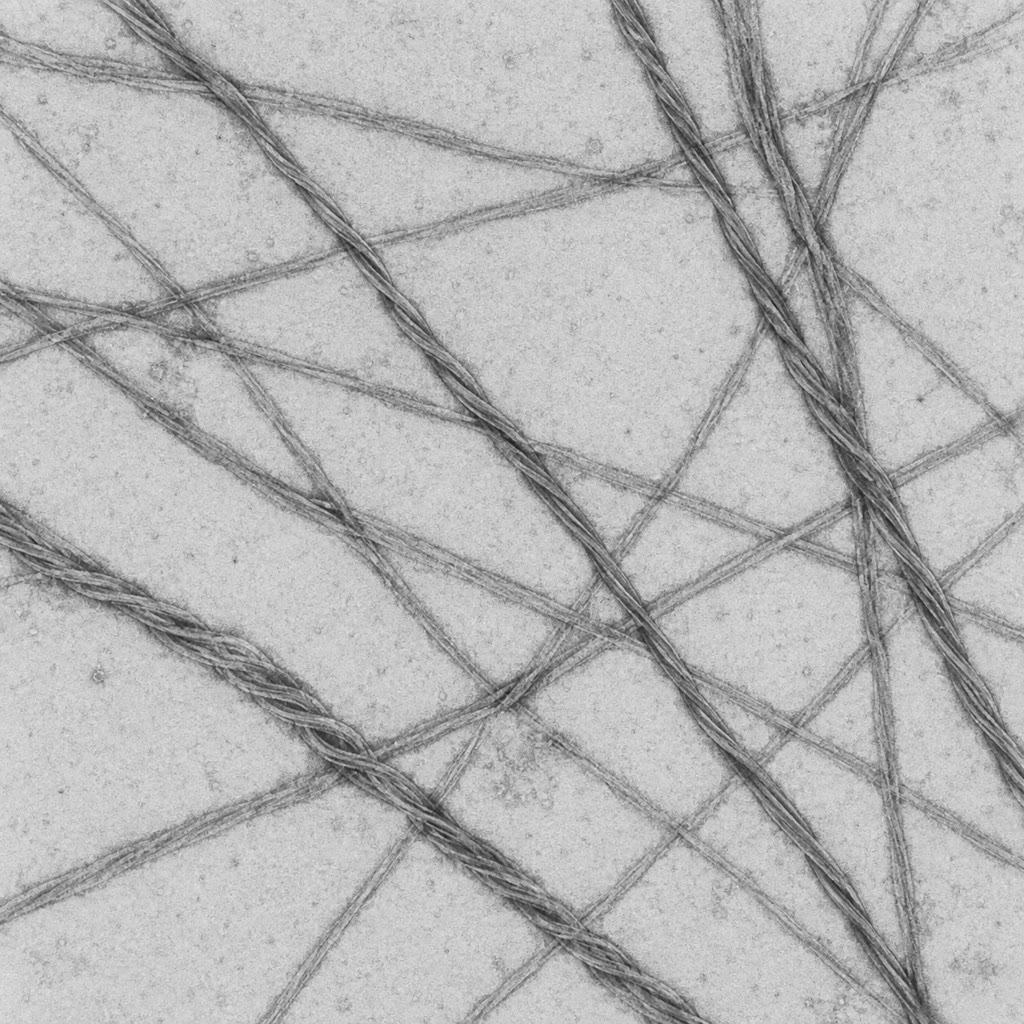
\includegraphics[width=0.36\linewidth]{images/book5/ai/b5-07-amyloid-fibrils.jpg}\hspace{0.04\linewidth}
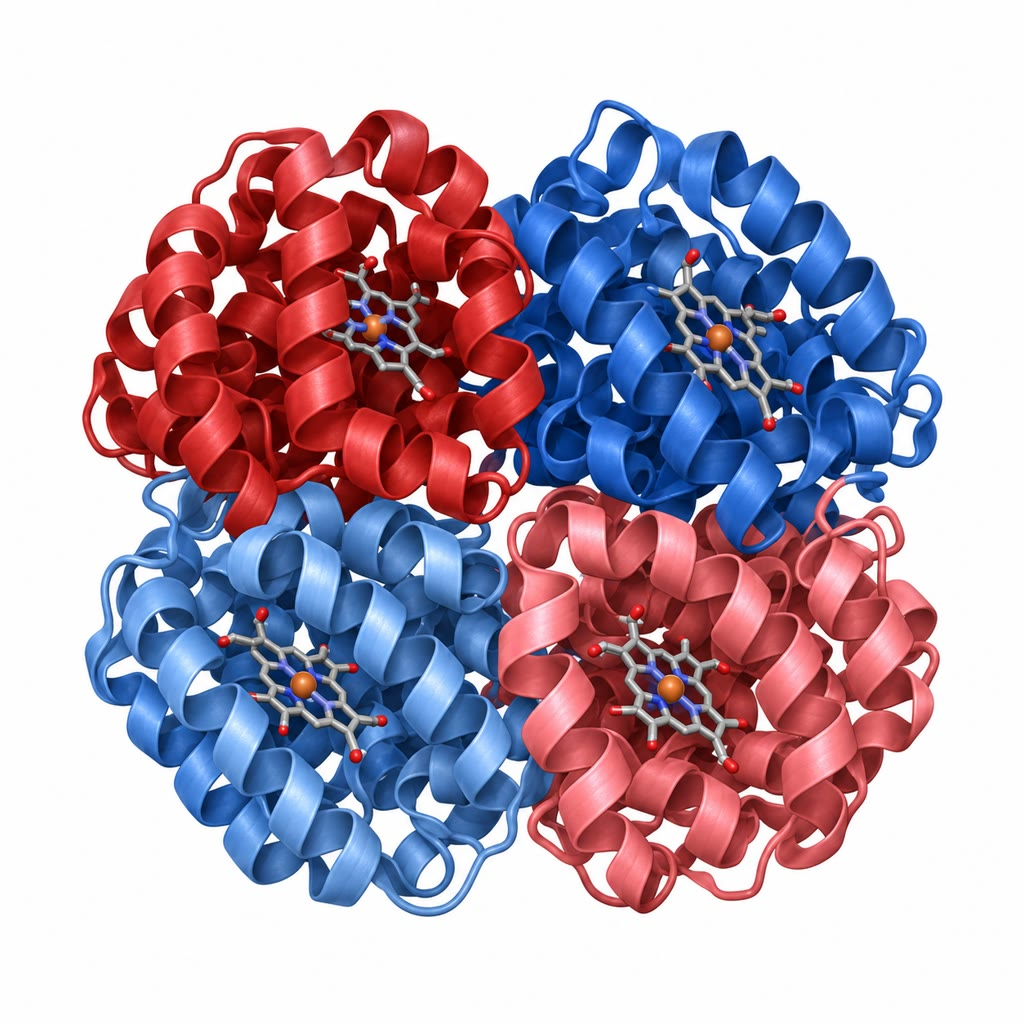
\includegraphics[width=0.36\linewidth]{images/book5/ai/b5-07-haemoglobin-model.jpg}

{\small 左：电子显微镜下的淀粉样纤维——笔直、
不分支、有时扭曲，无论由何种蛋白质构成，结构都相似。
右：血红蛋白四聚体，两条 $\alpha$ 链和两条
$\beta$ 链，每条链都容纳一个血红素。}
\end{omfigure}

\section{观察蛋白质}

\begin{definition}[结构测定方法]\label{def:b3:structural-biology:methods}
\index{X 射线晶体学}\index{核磁共振谱}\index{冷冻电子显微镜}\index{分辨率}
\emph{X 射线晶体学}先让蛋白质生长出晶体，
用 X 射线束照射，并记录衍射图样；
衍射斑点的位置给出晶格，其强度在恢复波的相位后
给出晶胞的电子密度，
据此搭建肽链。\emph{核磁共振}
（NMR）在溶液中测量空间上相邻
原子核之间的耦合，由此计算距离，进而得到结构；
它适用于约 \qty{40}{kDa} 以下的蛋白质，
并能揭示其运动。\emph{冷冻电子显微镜}对
数以千计至数百万个包埋于薄层玻璃态冰中的单分子成像，
每个分子取向随机，再将它们组合以重建三维密度；
自 2013 年直接电子探测器问世以来，它已能达到原子分辨率，
且无需晶体，因此大型复合体、膜蛋白以及
从未能结晶的柔性\omterm{def:b3:genomics:assembly}{组装}体如今都能常规解析。
结构的\emph{分辨率}是两个特征能被区分开的最小间距：
在 \qty{0.35}{nm} 时可确定主链和较大侧链的位置，
在 \qty{0.2}{nm} 时可确定每一个原子，
在 \qty{0.1}{nm} 时可确定氢原子。
\end{definition}

\begin{proof}[证据]
肯德鲁（1958）得到了第一个蛋白质结构，即抹香鲸
肌红蛋白，\omterm{def:b3:structural-biology:methods}{分辨率}为 \qty{0.6}{nm}——一根出乎意料地不规则的“香肠”，
“比任何人预测的都更复杂、对称性更差”
——1960 年，\omterm{def:b3:structural-biology:methods}{分辨率}达到 \qty{0.2}{nm} 时，
首次观察到了鲍林于 1951 年由模型搭建所提出的 $\alpha$ 螺旋。
佩鲁茨（1960）以 \qty{0.55}{nm} 的\omterm{def:b3:structural-biology:methods}{分辨率}解析了血红蛋白，
所用的是他为求相位而设计的重原子法：
与蛋白质结合的汞原子会改变衍射强度，
从而揭示缺失的信息。比较氧合与脱氧形式（1970 年），
他观察到结合氧时亚基彼此相对转动，
转角为 \qty{15}{\degree}，这是首次在原子尺度上
观察到的别构转变。
\end{proof}

\begin{omfigure}
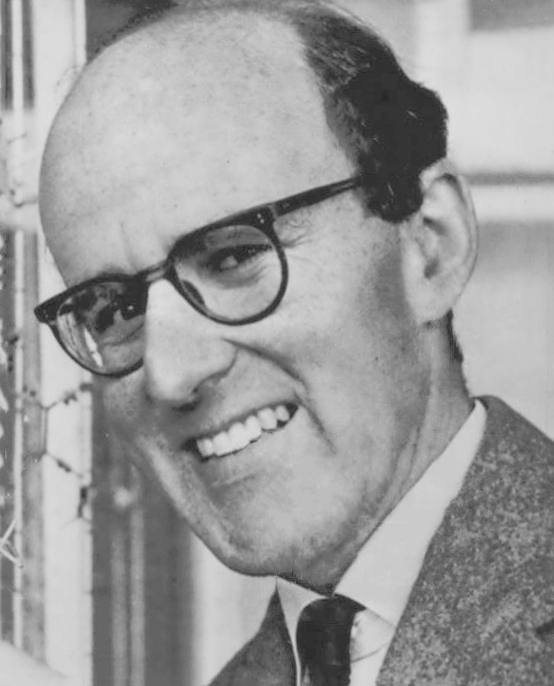
\includegraphics[width=0.30\linewidth]{images/book5/perutz.jpg}\hspace{0.04\linewidth}
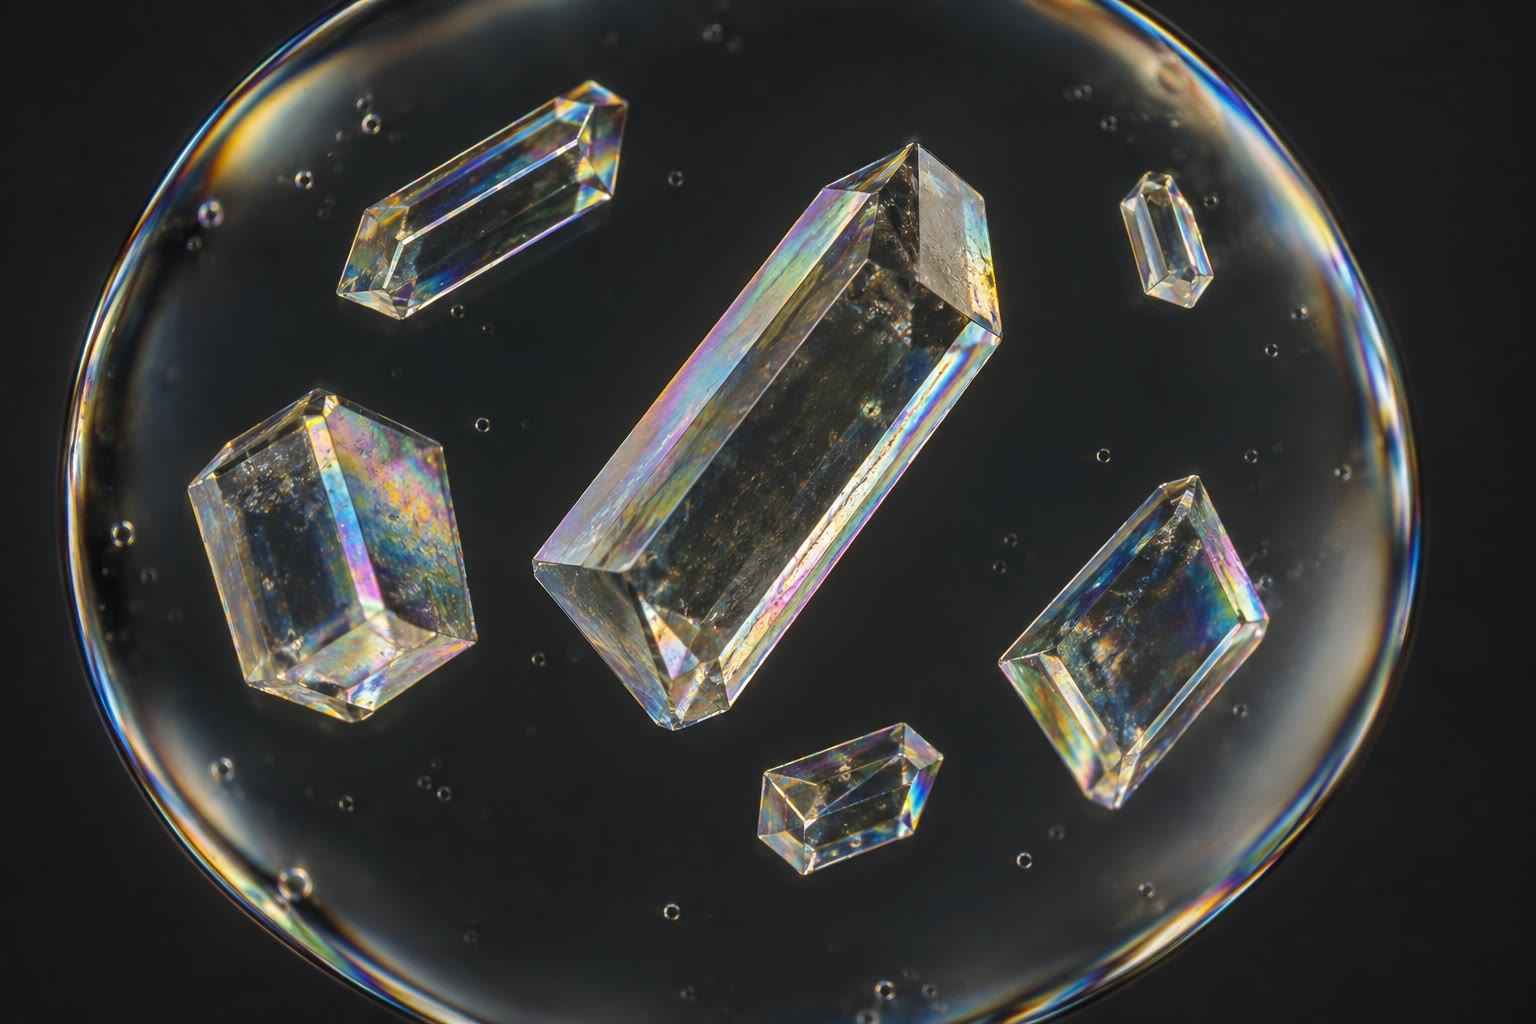
\includegraphics[width=0.30\linewidth]{images/book5/ai/b5-07-protein-crystals.jpg}\hspace{0.04\linewidth}
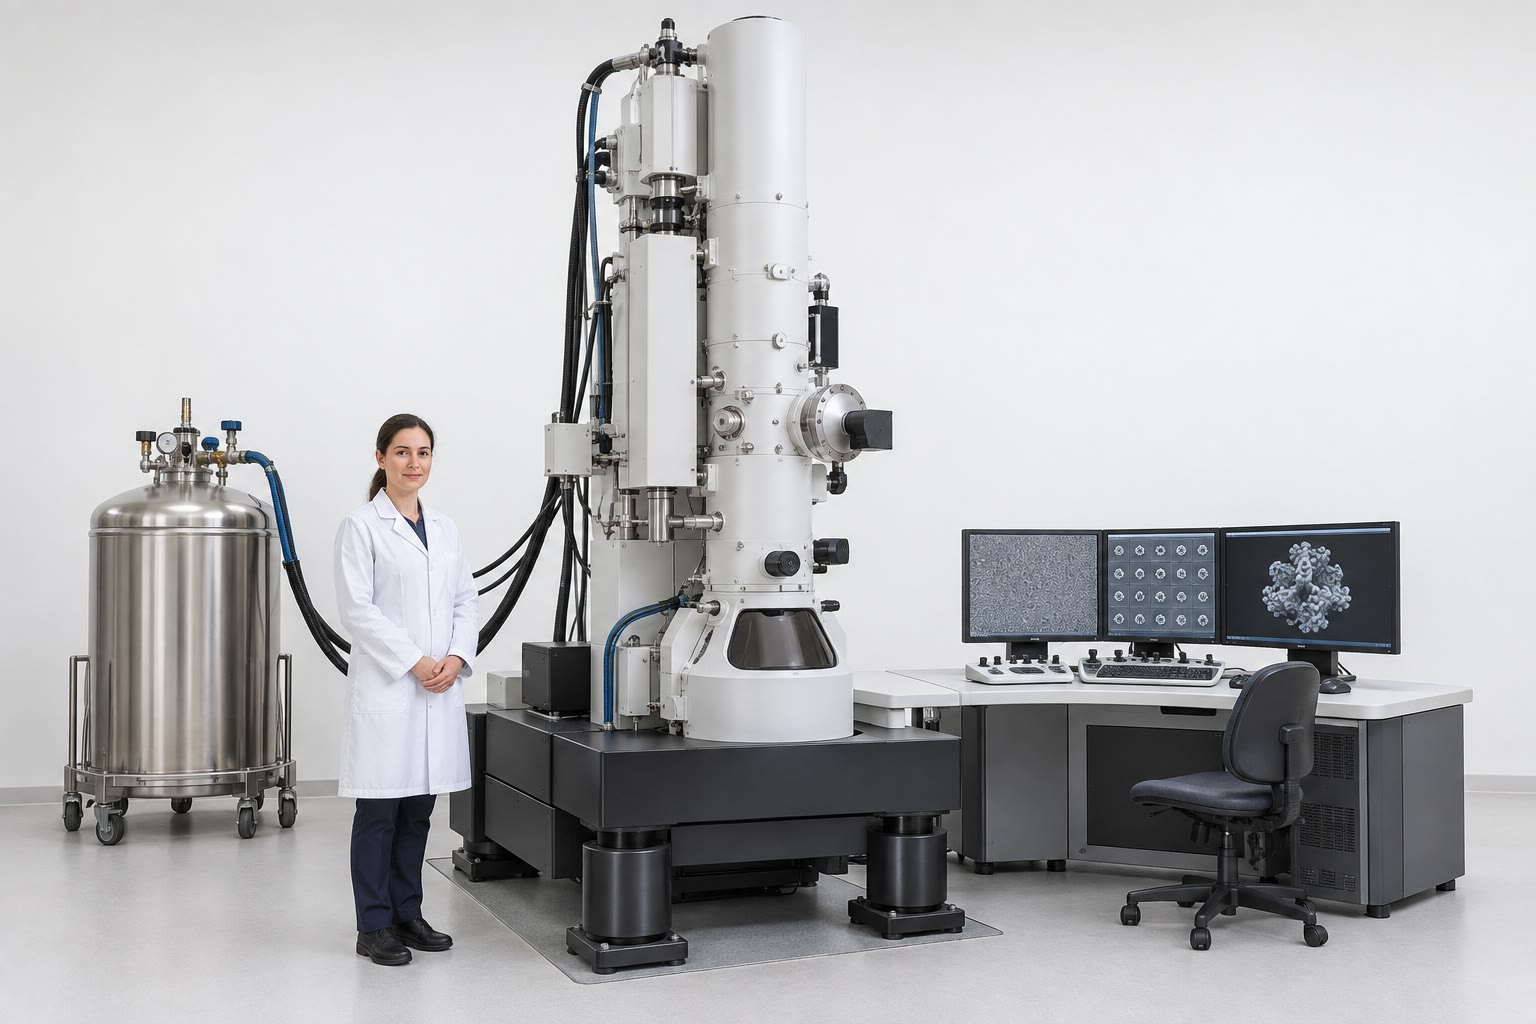
\includegraphics[width=0.30\linewidth]{images/book5/ai/b5-07-cryo-em.jpg}

{\small 1962 年的马克斯·佩鲁茨，同年因血红蛋白结构获诺贝尔奖
（美联社，公有领域）。中图：
悬滴中的蛋白质晶体，即晶体学的起点。右图：
\omterm{def:b3:structural-biology:methods}{冷冻电子显微镜}，这一仪器
使晶体不再必要。}
\end{omfigure}

\begin{method}[用晶体学解析结构]\label{met:b3:structural-biology:crystallography}
\index{布拉格定律}\index{相位问题}
（1）纯化数毫克蛋白质，并在数百种条件下
（沉淀剂、pH、盐）中筛选晶体；（2）将晶体速冻，
在同步辐射光源处收集衍射图像，晶体在光束中旋转；
（3）标定衍射斑点，得到晶胞与对称性；可见斑点的最大角度，
由布拉格定律 $d =
\lambda/(2\sin\theta)$ 决定\omterm{def:b3:structural-biology:methods}{分辨率}；（4）解决\emph{相位问题}——
探测器只记录强度而不记录相位——借助重原子，借助
硒代甲硫氨酸中硒的反常散射，或者对于
与某一已知蛋白质相似者，借助分子置换，将已知模型置于
晶胞中；（5）计算电子密度，
在其中搭建肽链，并对照数据精修模型，直至偏差
（$R$ 因子）足够小；（6）验证：几何构型、拉氏图离群点，
以及模型未参与精修的数据拟合情况。
\end{method}

\begin{omfigure}
\begin{tikzpicture}[every node/.style={font=\scriptsize}, >=stealth]
  % crystal
  \draw[thick, fill=omDef!20] (0,0) -- (1.4,0) -- (1.9,0.6) -- (0.5,0.6) -- cycle; \draw[thick, fill=omDef!30] (0,0) -- (0.5,0.6) -- (0.5,1.6) -- (0,1.0) -- cycle; \draw[thick, fill=omDef!25] (0.5,0.6) -- (1.9,0.6) -- (1.9,1.6) -- (0.5,1.6) -- cycle;
  \node[below] at (0.95,-0.1) {晶体：$10^{12}$ 个分子有序排列};
  % beam
  \draw[->, very thick, omThm] (-2.2,0.9) -- (-0.1,0.9); \node[above] at (-1.2,0.95) {X 射线，$\lambda \approx \qty{0.1}{nm}$};
  % diffracted beams
  \foreach \a in {-25,-12,5,18,30} \draw[->, omThm, thick] (1.9,0.9) -- ++(\a:3.2);
  % detector
  \draw[thick] (5.2,-1.2) rectangle (5.6,3.0); \node[right, align=left] at (5.7,2.6) {探测器：斑点位于 \\角度 $\theta$ 处，\\强度为 $I$};
  \foreach \y in {-0.6,-0.1,0.6,1.2,1.9,2.4} \fill[black] (5.4,\y) circle (0.06);
  % arrow to density
  \draw[->, very thick] (7.4,0.9) -- (8.6,0.9) node[midway, above, align=center] {相位 \\恢复};
  \node[right, align=left] at (8.7,1.4) {电子密度};
  \draw[omDef, thick] (8.8,0.4) .. controls (9.1,1.1) and (9.5,0.2) .. (9.8,0.8) .. controls (10.1,1.3) and (10.4,0.3) .. (10.7,0.9);
  \node[right, align=left] at (8.7,-0.4) {模型搭建其中、\\精修、验证};
  % Bragg
  \node[anchor=north west, align=left] at (-2.2,-0.7) {布拉格：$2d\sin\theta = \lambda$——\\所观测到的最大 $\theta$ 决定分辨率 $d$};
\end{tikzpicture}

{\small 由晶体到模型。规则晶格将 X 射线散射为
离散斑点；最大角度处的斑点决定\omterm{def:b3:structural-biology:methods}{分辨率}；
恢复相位后，强度转化为电子密度图，
在其中搭建肽链。}
\end{omfigure}

\begin{remark}[预测已进入方法之列]\label{rem:b3:structural-biology:prediction}
自 2020 年起，蛋白质结构可由其序列预测，准确度常可与
\qty{0.3}{nm} 的实验结构相媲美
（见\cref{ch:b3:bioinformatics}）。预测是对一种静态天然态的假说；
实验方法仍是最终的裁决者，
并且是关于配体、构象变化、
复合体与下文讨论的动力学信息的唯一来源。两者的角色已经改变——
预测模型借分子置换解决相位问题，
并指导哪些实验值得去做——而非
一方取代另一方。
\end{remark}

\section{别构作用：以血红蛋白为模型}

\begin{definition}[别构作用与协同性]\label{def:b3:structural-biology:allostery}
\index{别构作用}\index{协同性}\index{希尔系数}\index{T 态}\index{R 态}
若蛋白质中某一位点结合配体，
便会经由贯穿分子的构象变化改变另一位点的亲和力，
则称该蛋白质为\emph{别构}的。当两个位点结合
同一配体且效应为正时，结合称为
\emph{协同的}：饱和度分数 $Y$ 随配体浓度升高，
呈 S 形而非双曲线，经验上可由\emph{希尔方程}
$Y = [S]^{n_{H}}/(K^{n_{H}} +
[S]^{n_{H}})$ 描述，其中\emph{希尔系数} $n_{H} > 1$（血红蛋白：
$n_{H} \approx 2.8$，即四个位点；肌红蛋白仅一个位点：$n_{H} =
1$）。血红蛋白以两种四级构象存在，即
\emph{T 态}（紧张态，低亲和力，无氧结合时更为稳定）
与\emph{R 态}（松弛态，高亲和力）；二者
整体相互转换；质子、二氧化碳和 \omterm{prop:b3:structural-biology:mechanism}{2,3-二磷酸甘油酸}稳定 T 态，
从而降低亲和力——即\omterm{prop:b3:structural-biology:mechanism}{玻尔效应}，
工作中的组织酸性较强且温度较高，从血液中摄取更多氧气。
\end{definition}

\begin{theorem}[莫诺–怀曼–尚热模型]\label{thm:b3:structural-biology:mwc}
\index{莫诺–怀曼–尚热模型}\index{协同模型}
设一种蛋白质含 $n$ 个相同位点，存在两种构象，
$T$ 与 $R$，无配体时二者处于平衡，$L = [T_{0}]/[R_{0}]$，
$R$ 的每个位点与配体结合，解离常数为
$K_{R}$，$T$ 的每个位点则为 $K_{T}$，$c = K_{R}/K_{T} < 1$。
分子的全部位点同时切换（该转变称为
\emph{协同转变}）。令 $\alpha = [S]/K_{R}$，
则饱和度分数为
\[
Y = \frac{\alpha(1+\alpha)^{n-1} + Lc\alpha(1+c\alpha)^{n-1}}
{(1+\alpha)^{n} + L(1+c\alpha)^{n}},
\]
处于 $R$ 态的分子所占比例为 $\bar R =
(1+\alpha)^{n}/\bigl[(1+\alpha)^{n} + L(1+c\alpha)^{n}\bigr]$。当 $L
\gg 1$ 且 $c \ll 1$ 时，曲线呈 S 形：最初的配体
结合于数量稀少、高亲和力的 $R$ 分子，打破平衡，使得
结合又招募更多 $R$，其余位点的亲和力随之升高
——无需位点之间的任何直接相互作用即可实现\omterm{def:b3:structural-biology:allostery}{协同性}。
\end{theorem}
\begin{proof}
结合 $i$ 个配体、呈 $R$ 形式的物种，其浓度为
$[R_{0}]\binom{n}{i}\alpha^{i}$（$\binom{n}{i}$ 种占位方式中的每一种
依质量作用定律贡献 $([S]/K_{R})^{i}$），
在 $T$ 形式中则为 $[T_{0}]\binom{n}{i}(c\alpha)^{i}$，因为
$[S]/K_{T} = c\alpha$。对 $i$ 求和，由二项式定理可得
蛋白质总量为 $[R_{0}]\bigl[(1+\alpha)^{n} + L(1+c\alpha)^{n}\bigr]$，
结合的配体总量为 $[R_{0}]\sum_{i} i\binom{n}{i}\bigl[
\alpha^{i} + L(c\alpha)^{i}\bigr] = [R_{0}]\,n\bigl[\alpha(1+\alpha)^{n-1}
+ Lc\alpha(1+c\alpha)^{n-1}\bigr]$，其中用到 $\sum_{i} i\binom{n}{i}x^{i} =
nx(1+x)^{n-1}$。以结合配体量除以 $n$ 倍的蛋白质总量，即得
$Y$；$R$ 所占比例即 $R$ 项除以总和。当 $\alpha$
较小时，分母主要由 $T$ 项构成（因为 $L \gg 1$），
$Y \approx c\alpha$，即低 $T$ 亲和力；当 $\alpha$ 足够大时，
使得 $(1+\alpha)^{n} > L(1+c\alpha)^{n}$ 时，$R$ 项占了主导，
亲和力为 $K_{R}$：两种区间之间的转换即为 S 形曲线。
\end{proof}

\begin{example}[血红蛋白的数值示例]\label{ex:b3:structural-biology:hb-numbers}
取 $n = 4$，$K_{R} = \qty{1}{mmHg}$，$c = 0.01$（于是 $K_{T} =
\qty{100}{mmHg}$），$L = 3\times 10^{5}$。在
动脉血中的氧分压 \qty{100}{mmHg} 下，$\alpha = 100$，$Y =
0.97$；在静息时的静脉血值 \qty{40}{mmHg} 下，$Y = 0.78$；在
\qty{26}{mmHg} 下，$Y = 0.52$——该模型再现了半饱和
分压 \qty{26}{mmHg}；在运动肌肉中、\qty{20}{mmHg} 下
$Y = 0.35$。一种具有相同的
半饱和分压的非协同载体，在肺中将给出 $100/126 = 0.79$，
在肌肉中给出 $20/46 = 0.43$，其卸载量为容量的 $0.36$，
而血红蛋白卸载了 $0.62$。\omterm{def:b3:structural-biology:allostery}{协同性}正是使载体
能在一个压力下充分装载、而在仅低五倍的压力下大部分卸载
的原因。
\end{example}

\begin{omfigure}
\begin{tikzpicture}
\begin{axis}[
  width=0.7\linewidth, height=5.8cm,
  axis x line=bottom, axis y line=left,
  xmin=0, xmax=120, ymin=0, ymax=1.05,
  xlabel={氧分压 (mmHg)}, ylabel={饱和度 $Y$},
  xlabel style={font=\small, at={(axis description cs:0.5,-0.12)}, anchor=north},
  ylabel style={font=\small},
  tick label style={font=\small}, xtick={0,20,40,60,80,100,120}, ytick={0,0.5,1},
  clip=false,
]
\addplot[very thick, omThm, domain=0.1:120, samples=120] {(x*(1+x)^3 + 300000*0.01*x*(1+0.01*x)^3)/((1+x)^4 + 300000*(1+0.01*x)^4)};
\addplot[very thick, omDef, domain=0:120, samples=60] {x/(x+26)};
\addplot[dashed, gray] coordinates {(26,0) (26,0.52)}; \addplot[dashed, gray] coordinates {(0,0.52) (26,0.52)};
\draw[gray, dashed] (axis cs:20,0) -- (axis cs:20,0.35); \draw[gray, dashed] (axis cs:100,0) -- (axis cs:100,0.97);
\node[font=\scriptsize, omThm, anchor=north west] at (axis cs:50,0.15) {血红蛋白（MWC，$n = 4$，$L = 3\times 10^{5}$，$c = 0.01$）};
\node[font=\scriptsize, omDef, anchor=north east] at (axis cs:118,0.72) {单位点，相同 $P_{50}$};
\node[font=\scriptsize, anchor=south] at (axis cs:20,1.0) {肌肉}; \node[font=\scriptsize, anchor=south] at (axis cs:100,1.0) {肺};
\end{axis}
\end{tikzpicture}

{\small 血红蛋白的氧饱和度，由莫诺–怀曼–尚热方程
依照示例参数算得（红色），与具有相同半饱和分压的
单位点载体（蓝色）相比。在肺与工作肌肉之间，
协同载体卸载的氧量
几乎是后者的两倍。}
\end{omfigure}

\begin{proposition}[开关的机制]\label{prop:b3:structural-biology:mechanism}
\index{玻尔效应}\index{2,3-二磷酸甘油酸}
在脱氧血红蛋白中，铁原子略微位于血红素平面之外，
被近端组氨酸拉向一侧，血红素呈穹顶状。氧
的结合使血红素变平，并将铁原子连同
与之相连的组氨酸及其所在的螺旋一起，朝血红素方向拉近约 \qty{0.06}{nm}；
这一位移在两个二聚体之间的界面处被放大，
即 $\alpha_{1}\beta_{1}$ 与 $\alpha_{2}\beta_{2}$ 二聚体，它们旋转
\qty{15}{\degree}，并打破维持 T 态的盐桥。
效应物作用于这些相同的盐桥：质子结合在仅于 T 态中存在盐桥的
组氨酸上（即\omterm{prop:b3:structural-biology:mechanism}{玻尔效应}），二氧化碳与
稳定 T 态的氨基末端形成氨基甲酸酯，而
\omterm{prop:b3:structural-biology:mechanism}{2,3-二磷酸甘油酸}——一种强负电性的小分子——位于 $\beta$ 链之间的
中央空腔中，该空腔仅在 T 态时足够宽敞。胎儿血红蛋白
含 $\gamma$ 链，后者结合该分子较弱，
其亲和力高于母体，并从
胎盘中夺取氧气。
\end{proposition}

\section{蛋白质的运动}

\begin{definition}[无序与动力学]\label{def:b3:structural-biology:disorder}
\index{内在无序蛋白质}\index{构象系综}\index{生物分子凝聚体}
\emph{内在无序}区域本身不具有稳定的折叠结构，
以快速相互转换的构象系综形式存在，
常常只有在遇到结合伴侣时才折叠；约三分之一的人类蛋白质
含有超过三十个残基的无序区域。它们在信号传导与调控中
大量富集，其中柔性片段
可在多个位点被磷酸化，依次结合数个伴侣，
并起连接作用。折叠蛋白质同样会运动：侧链
在皮秒量级上旋转，环区在纳秒至微秒量级内打开，
\omterm{def:b3:structural-biology:levels}{结构域}在微秒至毫秒量级内发生铰链式运动，而酶的
催化循环是由此类运动编排而成的过程，而非静态的
锁钥模型。晶体结构只是一个
\emph{构象系综}的一张快照；核磁共振和分子模拟
则能看到其余部分。多价的无序蛋白质与 RNA 也能从细胞质中
分相，形成液滴——\emph{生物分子凝聚体}，例如
核仁、应激颗粒和 P 小体——它们
无需膜即可富集反应物，而这些凝聚体
老化为固态聚集体，是通向淀粉样疾病的一条途径。
\end{definition}

\begin{remark}[结构与功能]\label{rem:b3:structural-biology:sf}
六十年结构研究的启示是双重的。折叠方式是
对某一物理问题的解答——结合此物、催化彼反应、在四纳米范围内传递信号——
而了解结构往往能使机制一目了然，正如血红素中铁原子的情况
以及血红蛋白二聚体在氧驱动下的旋转所示。折叠方式
也是历史的产物：同样的几百种结构型式经过修补、
复制与融合，服务于蛋白质功能的全部多样性，
因此，细菌蛋白质的结构
常常能告诉人们，
其人类同源物如何工作。
\end{remark}

\section{练习}

\begin{exercise}[$\star$]\label{exo:b3:structural-biology:1}
定义蛋白质结构的四个层次，并
分别举出血红蛋白中各层次的实例。
\end{exercise}

\begin{exercise}[$\star$]\label{exo:b3:structural-biology:2}
一个 $\alpha$ 螺旋含有 $36$ 个残基。求其长度，
它形成多少个转角，以及有多少个主链氢键维系它
（每个残基的羰基与其后第四个残基的酰胺基形成氢键）。
\end{exercise}

\begin{exercise}[$\star$]\label{exo:b3:structural-biology:3}
安芬森对核糖核酸酶的复性实验说明了什么，
以及为何在不含任何细胞成分的条件下进行该实验十分重要？
\end{exercise}

\begin{exercise}[$\star$]\label{exo:b3:structural-biology:4}
将 X 射线晶体学、核磁共振和\omterm{def:b3:structural-biology:methods}{冷冻电子显微镜}，
按各自最适宜处理的蛋白质大小排序，
并说明哪一种方法能提供关于运动的信息。
\end{exercise}

\begin{exercise}[$\star\star$]\label{exo:b3:structural-biology:5}
重算莱文塔尔计数：对含 $150$ 个残基、$k = 2$ 的蛋白质，
以及含 $20$ 个残基、$k = 3$ 的肽，
以每秒 $10^{12}$ 次尝试的速率，两者中哪一个
可以设想在一秒内通过随机搜索完成？
\end{exercise}

\begin{exercise}[$\star\star$]\label{exo:b3:structural-biology:6}
利用 MWC 方程，取 $n = 2$、$L = 100$、$c = 0.01$，计算
$Y$ 在 $\alpha = 1$、$10$ 和 $100$ 时的值，并与单一位点的
解离常数 $K_{R}$（$Y = \alpha/(1+\alpha)$）作比较。\omterm{def:b3:structural-biology:allostery}{协同性}
在何处体现？
\end{exercise}

\begin{exercise}[$\star\star$]\label{exo:b3:structural-biology:7}
用 MWC 模型解释，为何 \omterm{prop:b3:structural-biology:mechanism}{2,3-二磷酸甘油酸}会降低
血红蛋白的氧亲和力，它改变了模型的哪个参数，
以及失去该化合物的储存血液，为何在输血时
向受血者输送氧气的效果较差。
\end{exercise}

\begin{exercise}[$\star\star$]\label{exo:b3:structural-biology:8}
一块晶体以最大角 $\theta = \qty{15}{\degree}$ 发生衍射，
所用 X 射线波长为 \qty{0.1}{nm}。\omterm{def:b3:structural-biology:methods}{分辨率}是多少？蛋白质的哪些
特征能够被观察到？
若波长为 \qty{0.12}{nm}，则需要多大的角度？
\end{exercise}

\begin{exercise}[$\star\star$]\label{exo:b3:structural-biology:9}
一次突变将埋藏的亮氨酸替换为赖氨酸，
利用\cref{prop:b3:structural-biology:forces}预测其对稳定性的影响，
并解释为何同一取代若发生在表面则无害。
再解释，为何 $\Delta G_{\text{折叠}} =
\qty{-30}{kJ/mol}$ 的蛋白质并不“很稳定”，
尽管这一数值看起来很大。
\end{exercise}

\begin{exercise}[$\star\star\star$]\label{exo:b3:structural-biology:10}
推导处于 $R$ 态的分子比例 $\bar R$，
由\cref{thm:b3:structural-biology:mwc}证明中计数的分子种类出发，
并证明当 $c \to 0$ 时，使半数分子处于 $R$ 态的配体浓度
满足 $(1+\alpha)^{n} = L$。取血红蛋白的参数，计算
该 $\alpha$ 的值，并与 $P_{50}$ 比较。
\end{exercise}

\begin{exercise}[$\star\star\star$]\label{exo:b3:structural-biology:11}
\omterm{def:b3:structural-biology:amyloid}{朊病毒}传递的是一种构象。试解释为何“仅蛋白质”假说
曾遭到抵制，哪一项实验可以否定它，以及哪些证据
（感染性对核酸酶和紫外线的抗性、对蛋白质变性剂的
敏感性、人工合成的\omterm{def:b3:structural-biology:amyloid}{朊病毒}）支持该假说。为何\omterm{def:b3:structural-biology:amyloid}{朊病毒}
需要一个种子？
\end{exercise}

\begin{exercise}[$\star\star\star$]\label{exo:b3:structural-biology:12}
某一蛋白质家族保持了其\omterm{def:b3:structural-biology:levels}{折叠类型}，而其序列的一致性
已降至 \qty{15}{\%}。试解释为何结构比序列更为保守，
被保守的残基属于哪一类，以及这一事实如何既被
谱方法（\cref{ch:b3:bioinformatics}）所利用，
也被新蛋白质的设计所利用。
\end{exercise}

\section{问题：珠蛋白的折叠}

\begin{problem}[{周末问题——测量珠蛋白的螺旋，将其折叠时间与莱文塔尔估计相比，
由双态模型计算其氧结合，并由晶体解出其结构，
最后讨论肺与肌肉之间的饱和度差、
莱文塔尔时间以及
该图的分辨率}]
\label{pb:b3:structural-biology:1}
数据：一条含 $150$ 个残基的珠蛋白链，平均残基质量为 \qty{110}{Da}，
其中 \qty{75}{\%} 的残基位于八个 $\alpha$ 螺旋中；螺旋的每残基轴向上升
\qty{0.15}{nm}，每圈 $3.6$ 个残基。蛋白质的偏比容为 \qty{0.73}{cm^3/g}。
血红蛋白的 MWC 参数为：$n = 4$，$K_{R} = \qty{1}{mmHg}$，$c = 0.01$，$L = 3\times 10^{5}$。
X 射线波长为 \qty{0.1}{nm}；
晶胞为棱长 \qty{6}{nm} 的立方体；
晶体为棱长 \qty{100}{\micro m} 的立方体。

\medskip
\noindent\textbf{第一部分——链的结构剖析。}
\begin{enumerate}
  \item 螺旋中有多少个残基？螺旋的总长度为多少，
        共形成多少个转角？
  \item 螺旋中共含多少个主链氢键，
        每条螺旋中，超出前四个的每个残基计为一个？
  \item 求该链的质量，并由偏比容求其体积；
        求体积与该球体积相等的球的半径。
  \item 设伸展的链每个残基长 \qty{0.36}{nm}，
        将其长度与球的直径比较，
        折叠将链压缩了多少倍？
  \item 八条螺旋平均各含 $14$ 个残基。若将全部残基首尾相接排列，
        则螺旋部分占伸展长度的比例为多少？
        螺旋如何使链缩短？
  \item 一个珠蛋白的核心埋藏约 $40$ 个非极性侧链。
        取每个埋藏侧链的疏水稳定化能为 \qty{4}{kJ/mol}，
        并取折叠时每残基的构象熵代价为
        \qty{0.9}{kJ/mol}（全部 $150$ 个残基），
        估算折叠的净 $\Delta G$，并与
        \cref{prop:b3:structural-biology:forces}中的范围比较。
\end{enumerate}

\medskip
\noindent\textbf{第二部分——寻找折叠方式。}
\begin{enumerate}[resume]
  \item 计算 $150$ 个残基在 $k = 3$ 时的莱文塔尔计数，
        以及以每秒 $10^{12}$ 次的速率抽样所需的时间。
  \item 珠蛋白在 \qty{10}{ms} 内折叠。它至多可能访问过
        多少种构象？这占全部计数的多大比例？
  \item 若改设每个螺旋独立地在
        \qty{1}{\micro s} 内形成，随后八个已形成的螺旋
        在 $8!$ 种排列中寻找其堆积方式，抽样速率为每秒 $10^{6}$ 次。
        估算折叠时间。这是否为漏斗？
  \item \omterm{def:b3:structural-biology:chaperones}{伴侣蛋白}每个循环包裹一条链 \qty{10}{s}，
        并以每次循环 $0.3$ 的概率将其释放为折叠态。求
        折叠一个难折叠底物所需的期望循环数与期望时间，
        以及一分钟后仍未折叠的比例
        为多少？
  \item 一个降低稳定性的突变使未折叠比例在
        \qty{37}{\celsius} 时由 $10^{-4}$ 升至 $10^{-2}$。取 $\Delta G =
        -RT\ln(K)$，$K = [\text{折叠态}]/[\text{未折叠态}]$，则
        $\Delta G_{\text{折叠}}$ 变化了多少？
  \item 利用聚集需要种子这一点，解释为何未折叠蛋白多出一百倍
        便足以造成健康与\omterm{def:b3:structural-biology:amyloid}{淀粉样蛋白}病之间的差别。
        （淀粉样聚集需要一个种子。）
\end{enumerate}

\medskip
\noindent\textbf{第三部分——结合氧气。}
\begin{enumerate}[resume]
  \item 由 MWC 方程计算 $Y$ 在 $\alpha = 100$（肺）与
        $\alpha = 20$（工作肌肉）时的值。
  \item 计算在这两种压强下处于 $R$ 态的
        分子所占比例。
  \item 从肺到肌肉之间，已结合的氧气有多少被释放？
        请与半饱和压强为
        \qty{26}{mmHg} 的单位点载体相比较。
  \item 血液每升含 \qty{150}{g} 血红蛋白，每克血红蛋白
        可结合 \qty{1.34}{mL} 氧气。每升血液中血红蛋白
        可向肌肉输送多少毫升氧气（由第 15 题得出）？静息人体的
        耗氧速率为 \qty{250}{mL/min}，则静息时需要多大血流量
        （氧卸载由 $0.97$ 降至
        $0.78$）？
  \item 二磷酸甘油酸将 $L$ 提高到 $3\times 10^{6}$。重新计算
        $Y$ 在 $\alpha = 40$ 时的值，并说明此变化对
        静息时的输送有何影响。
  \item 胎儿血红蛋白实际上具有 $L = 3\times 10^{4}$。计算
        其在胎盘压强为 \qty{30}{mmHg} 时的 $Y$，
        与母体比较，并解释氧的转运过程。
\end{enumerate}

\medskip
\noindent\textbf{第四部分——观察结构。}
\begin{enumerate}[resume]
  \item 晶体包含多少个晶胞？若每个晶胞含四条珠蛋白链，
        则共同衍射的分子有多少个？
  \item 观察到的衍射斑点可见至 $\theta = \qty{14.5}{\degree}$。
        其\omterm{def:b3:structural-biology:methods}{分辨率}为多少，侧链能否被定位？
  \item 何种角度可给出 \qty{0.15}{nm}？晶体有序性差时，
        为何只能在小角度处发生衍射？
  \item 在\omterm{def:b3:structural-biology:methods}{冷冻电子显微镜}中，平均图像的信号
        随颗粒数的平方根生长。若
        \num{10000} 个颗粒给出 \qty{0.6}{nm}，且\omterm{def:b3:structural-biology:methods}{分辨率}
        随信号的倒数成比例改善，则需多少颗粒
        方可得到 \qty{0.3}{nm}？
  \item \omterm{def:b3:structural-biology:methods}{冷冻电子显微镜}无需晶体。列举两类
        蛋白质或复合体，对其能否获得结构起决定作用，
        并说明原因。
  \item 珠蛋白的预测模型在主链上平均与晶体结构
        相差 \qty{0.1}{nm}。列举预测无法提供、而晶体
        能够提供的两项内容。
  \item 概括：肺与肌肉之间的氧卸载（第 15 题）、
        $150$ 个残基的莱文塔尔时间（第 7 题）以及
        电子密度图的\omterm{def:b3:structural-biology:methods}{分辨率}（第 20 题）。
\end{enumerate}
\end{problem}
